In this chapter we introduce a novel pixel-based readout technology for TPCs.
Pixel based readouts offer several advantages over the traditional wire readout \citep{lartpc_recon_problems_joshi_2015}.
A key improvement offered is true 3-D image reconstruction.
This allows for sharper vertex reconstruction, thereby improving the overall resolution of DUNE and decreasing the required time for a NP measurement.
Other advantages are ease of data analysis and reduction in total data storage.
A pixel based readout automatically records two of the three spatial dimensions, and thereby provides for simpler analysis.
Additionally, the pixelated readout method presented here cuts the total required data storage and data acquisition rate (without loss to precision) by several orders of magnitude.

However, the advantages also come with the cost of increased design complexity as the number of readout channels increases by more than three orders of magnitude. 
The traditional wire based readout within a DUNE module will include hundreds to thousands of channels, whereas a full DUNE module with a pixel-based readout will have 10's of millions of channels.
This number of required channels to be stably readout during DUNE's expected lifetime ($> 10$ years), where the electronics continually operate at liquid argon temperatures is likely the largest hurtle for a pixel-based design.
The aim of this dissertation is to address the channel-size problem.

\section{Q-Pix: The Circuit Level Design}

The fundamental readout circuit~(\ref{fig:qpixCircuit}) was first introduced by Nygren and Mei~\citep{qpix:nygren:mei}.
The principle of the front-end circuit operates on measuring a schmitt trigger output connected to an integrating capacitor circuit.

The circuit input is connected to the anode of a TPC where drifted electron charge accumulates.
Voltage is then built up from the charge stored on the pixel based on the capacitance according to the equation:

\begin{equation}
Q_{i} = C_{i}V_{i}
\end{equation}

After the capacitor voltage ($V_{i}$) exceeds a set threshold value the schmitt trigger activates.
The trigger output is recorded by digital logic and also drives the reset of the integrator.
Since the capacitor reset happens at the same time as the issued trigger the digitally-recorded value is the reset time.

\begin{figure}[]
\centering
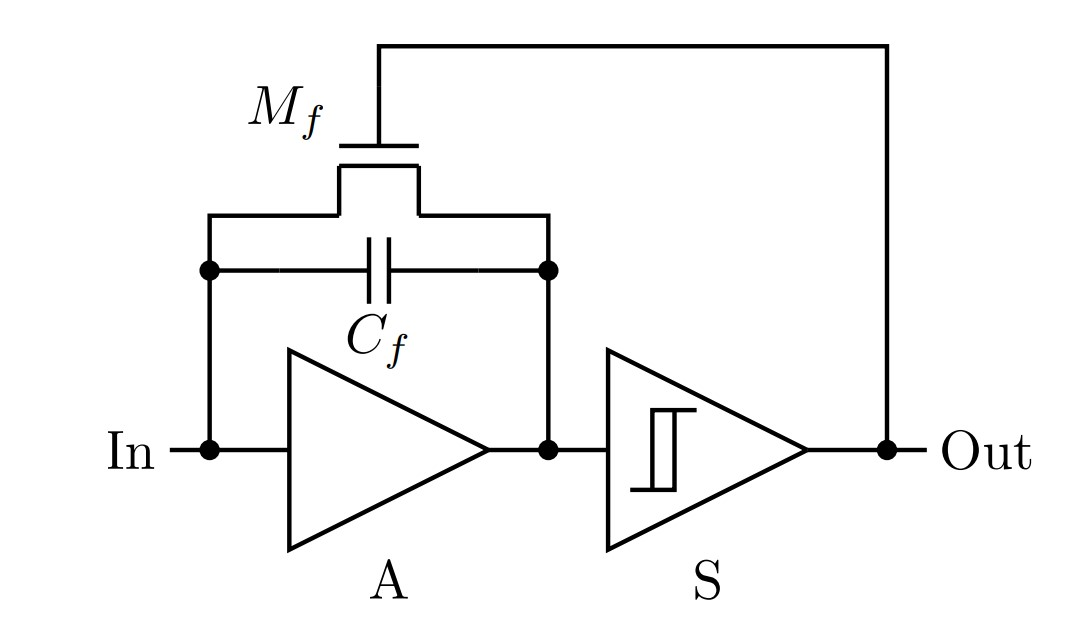
\includegraphics[width=\textwidth]{images/qpix_circuit.jpg}
\caption{Image of Basic Q-Pix Readout circuit. Currently this front-end circuit is being designed as custom analog ASIC which has 16 channels. Image is taken from \citep{qpix:nygren:mei}.}
\end{figure}
~\label{fig:qpixCircuit}

\subsection{Reconstructing Voltage from Time Resets}

Here we describe the basic principle of reconstructing the voltage measurement from a reset.
The key insight for this readout technology is that time (instead of charge) is the value that is recorded.
Therefore, recorded values happen only when there is enough charge to cause a reset which prevents long dead time measurements.
This concept follows the detector concept of least action in that all measurements are detector responses.

\begin{figure}[]
\centering
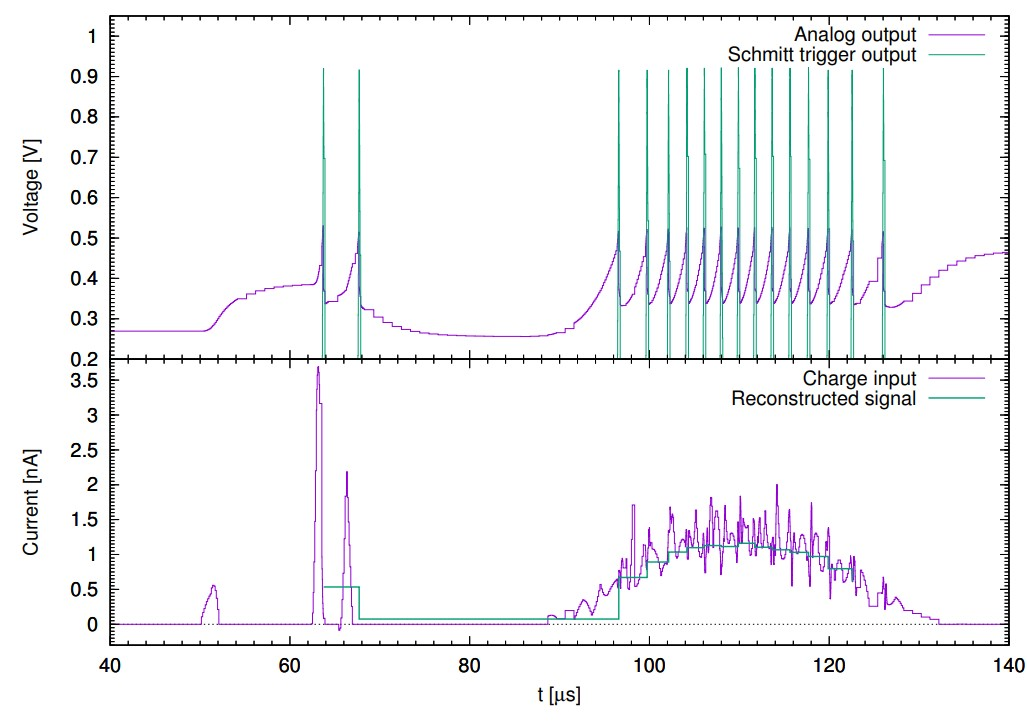
\includegraphics[width=\textwidth]{images/qpix_rtd_reconstruction_example.jpg}
\caption{Example reconstruction of the reset time difference (RTD) based on the Q-Pix readout design. Image is taken from \citep{qpix:nygren:mei}.}
\end{figure}
~\label{fig:qpixRecon1}

\begin{figure}[]
\centering
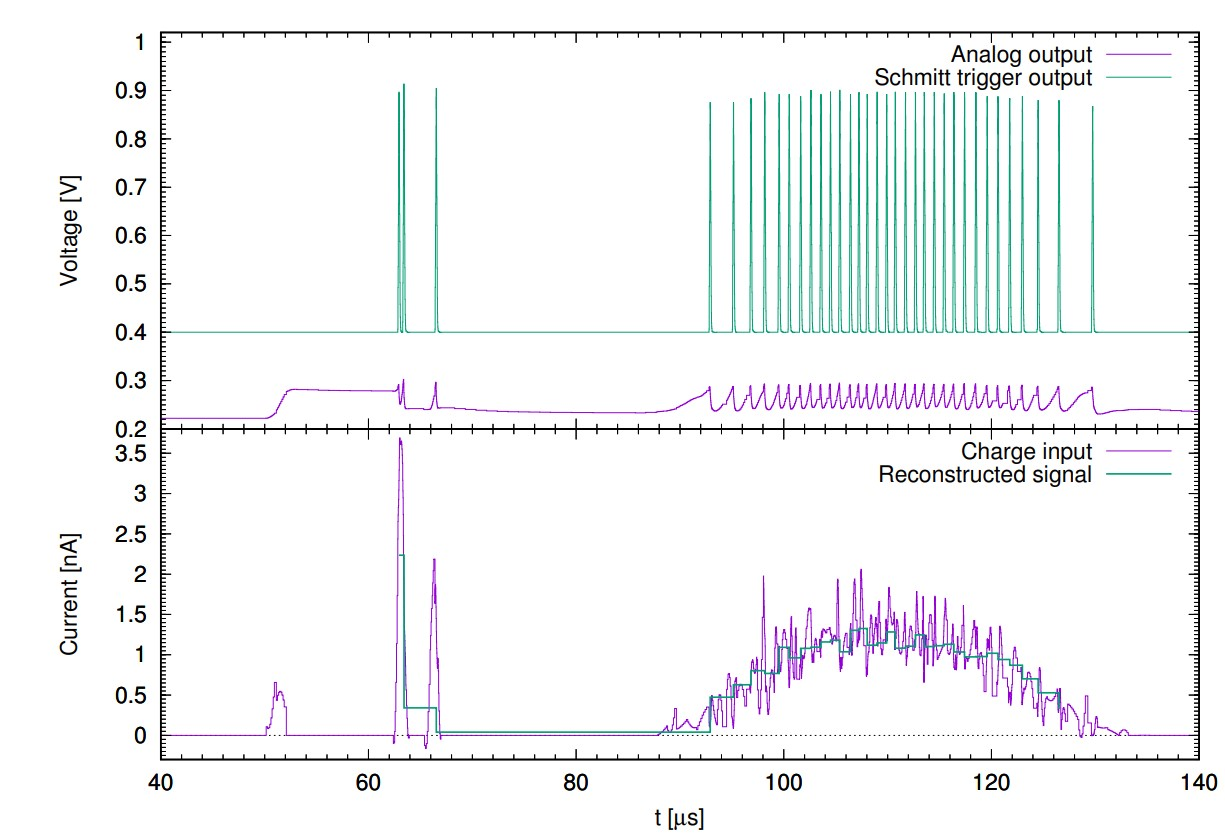
\includegraphics[width=\textwidth]{images/qpix_rtd_reconstruction_example_03fc.jpg}
\caption{Example reconstruction of the reset time difference (RTD) based on the Q-Pix readout design. delta-Q was chosen to be $0.3 fC$. Image is taken from \citep{qpix:nygren:mei}.}
\end{figure}
~\label{fig:qpixRecon2}


\subsubsection{Background Calibration}

Concept of this combined ASIC and reducing the number of channels relies on digital multiplexing.

The capacitance ($C_{i}$) for each pixel is a systematic which can be calibrated periodically using the background current from $Ar^{39}$ decay.

Once the trigger voltage ($V_{i}$) is exceeded the schmidt trigger issues the timing reset which is then recorded as a 32-bit digital timestamp.
This timestamp value is recorded against a free running local oscillator ($\approx$ 30 MHz).
The number of free running clocks in the entire system is expected to be the number of channels ($N_{c}$) divided by the number of digitally multiplexed channels ($N_{d}$), which are taken to be 16.

\subsection{Making a 3-D Image}

One of the important features of a TPC is the ability to reconstruct full 3-D images.
The intended benefit of a pixelated readout on any TPC is to show that there are improvements to reconstruction of these images.

In order to reconstruct the image of the interaction from a set of data above the pixel the required data are the reset time at a pixel i ($T_{ri}$), event time ($T_{e}$), and the pixel ID.
We assume that $T_{e}$ (as is normally used to tag events in TPCs) uses a trigger time from a secondary PMT system from the scintillation light produced by the interaction to tag an event of interest.
Since the scintillation photons travel much faster than the drift electrons, we can use the $T_{e}$ as the starting time.

The pixel ID of each reset gives two of the three remaining coordinates ($\hat{x}$ and $\hat{y}$).
The last coordinate ($\hat{z}$) is reconstructed using $T_{ri}$.

% average value is 1.6 mm / us from Nygren's QPix paper.
Since the drift velocity of the electrons ($v_{e}$) is constant in a TPC the distance that the electrons traveled to reach the anode plane ($\hat{z}$) is determined based on only the drift time:
\begin{equation}
  z = v_{e} * T_{drift}
\end{equation}~\label{eq:driftDistance}

However, this drift time is measured directly from the difference between the event time ($T_{e}$) and the reset time for this pixel ($T_{ri}$).
\begin{equation}
  T_{drift} = T_{ri} - T_{e}
\end{equation}

The drift distance in equation~(\ref{eq:driftDistance}) becomes:
\begin{equation}
  z = v_{e} * (T_{ri} - T_{e})
\end{equation}~\label{eq:driftDistanceCalc}

\subsubsection{Uncertainties}

Therefore the precision of the measurement of $\hat{z}$ is based on equation~\ref{eq:driftDistanceCalc}.
The uncertainty for the two transverse coordinates on the anode plane ($\hat{x}$ and $\hat{y}$) which are reasonable assumed to be uniform over the pixel are then $\frac{3 mm}{\sqrt{12}} \approx 0.87 mm$.


\subsection{Bad Scenarios}

Here we briefly describe potential issues of the readout circuit presented here.

\subsubsection{Maximum Reset Rate}



\section{System Requirements}

This differs from other concepts such as Genetic Multiplexing (\citep{PROCUREUR2013888_genetic_multiplexing}) and using only regions of interest (ROI).

Therefore, the total number of free running oscillators ($N_{osc}$) per DUNE-APA for a given pixel pixel of $3~mm^{2}$ is:

\begin{equation}
N_{osc} = \frac{6.3 * 2.5}{9*10^{-6}*16} = 109375
\end{equation}

Therefore we expect the order of the number of free running oscillators per DUNE-APA $\mathcal{O}$($10^5$).

\subsection{Single Point Failures}

\section{How Q-Pix fits into a DUNE APA}

DUNE Anode Plane Assemblies (APA) designs are based on \citep{DUNE-FD_TDRv4:Abi_2020}.

%% example image of DUNE-APA from DUNE-FD TDR.
\begin{figure}[]
\centering
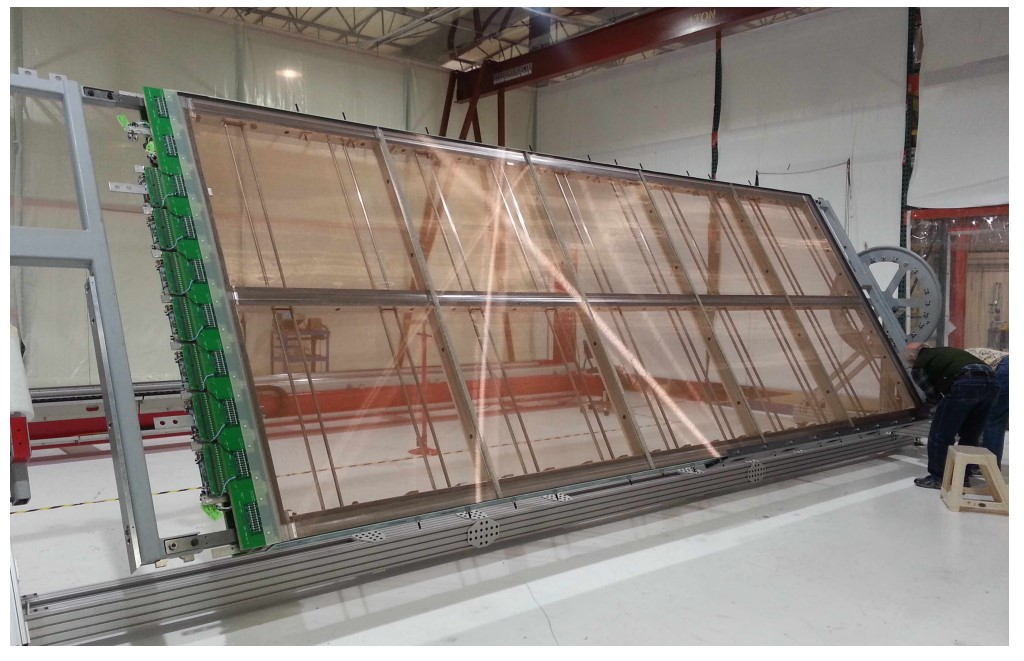
\includegraphics[width=\textwidth]{images/dune_fd_tdr_apa_image.jpg}
\caption{A simple caption \citep{DUNE-FD_TDRv4:Abi_2020}}
\end{figure}
